% =========================
% main.tex
% =========================
\documentclass[11pt]{article}

\usepackage[margin=1in]{geometry}
\usepackage{amsmath, amssymb}
\usepackage{graphicx}
\usepackage{booktabs}
\usepackage{enumitem}
\usepackage{hyperref}
\usepackage{xcolor}
\usepackage{caption}
\usepackage{subcaption}
\usepackage{tikz}
\usetikzlibrary{positioning, arrows.meta, shapes.geometric, calc}

\hypersetup{
  colorlinks=true,
  linkcolor=blue,
  citecolor=blue,
  urlcolor=blue
}

\title{\textbf{Beyond Imitation: Teaching Autonomous Cars to Drive (and Explain Themselves)}}
\author{\textit{Research Report -- Nawar Sgier}}
\date{}

\begin{document}
\maketitle

\begin{abstract}
End-to-End (E2E) autonomous driving has come a long way from simple lane-following. Today, we build complex ``brains'' that take raw sensor data and map it directly to the steering wheel and pedals.

A current heavyweight in this arena is TransFuser++ (TF++). It achieves strong CARLA benchmark results using Imitation Learning (IL)---watching an expert drive and copying them. But there is a catch: IL systems can lean on \emph{hidden biases} rather than learning robust, causal driving behavior. For example, dense GPS-like target points can act as a crutch for lateral recovery, and supervised regression can average multi-modal longitudinal futures (e.g., stop vs.\ go), creating hesitant behavior. On top of that, the policy is a black box: when it fails, it cannot clearly tell us why.

This report proposes a New Model that stops memorizing and starts \emph{optimizing}. It introduces four upgrades: (1) a ResNet-18 backbone for fast, reliable vision; (2) DistilBERT to accept natural-language commands; (3) Reinforcement Learning with PPO to learn from trial-and-error under an explicit safety reward; and (4) a GRU explainability head to generate short rationalizations in plain English. We formalize the key components, outline a CARLA evaluation protocol, and summarize projected results on Longest6.
\end{abstract}

% =========================================================
\section{The Big Picture}
% =========================================================

\subsection{Why TransFuser++ Is Strong (and Why It Can Still Be Fragile)}
TransFuser++ (TF++) is a high-performing E2E sensor-fusion agent in CARLA. It uses Imitation Learning (IL), typically Behavior Cloning (BC), to mimic an expert's actions. This can work extremely well on benchmarks, but the learned behavior may depend on shortcuts present in the training setup rather than stable driving rules.

Two examples of \emph{hidden biases}:
\begin{itemize}[leftmargin=1.2em]
  \item \textbf{GPS target-point shortcut:} steering toward dense, local GNSS-like target points can look like ``recovery'' without truly learning lane semantics.
  \item \textbf{Longitudinal averaging:} if the expert behavior is multi-modal (stop vs.\ go), regression can output an average (slow rolling / hesitation), which sometimes reduces collisions but is not a principled decision rule.
\end{itemize}

\subsection{What the New Model Changes}
We rebuild the system around four goals:
\begin{enumerate}[leftmargin=1.2em]
  \item \textbf{Fast, reliable perception:} ResNet-18 backbone for predictable latency.
  \item \textbf{Natural-language conditioning:} DistilBERT embeddings instead of one-hot command IDs.
  \item \textbf{Learning from experience:} PPO (RL) to reduce distribution shift and optimize safety rewards directly.
  \item \textbf{Explainability:} a GRU head that generates short, human-readable rationalizations.
\end{enumerate}

% =========================================================
\section{How We're Rebuilding the Architecture}
% =========================================================

\subsection{Overview}
At time $t$, the agent consumes:
\begin{itemize}[leftmargin=1.2em]
  \item \textbf{Visual input} $I_t$: a front RGB image ($H\times W$).
  \item \textbf{LiDAR input} $L_t$: a point cloud projected to a BEV grid / pseudo-image.
  \item \textbf{Command} $C_t$: a natural-language instruction string.
  \item \textbf{Vehicle state} $v_t$: ego speed (scalar).
\end{itemize}

Figure~\ref{fig:arch} shows the high-level design.

\begin{figure}[h]
\centering
\resizebox{\linewidth}{!}{%
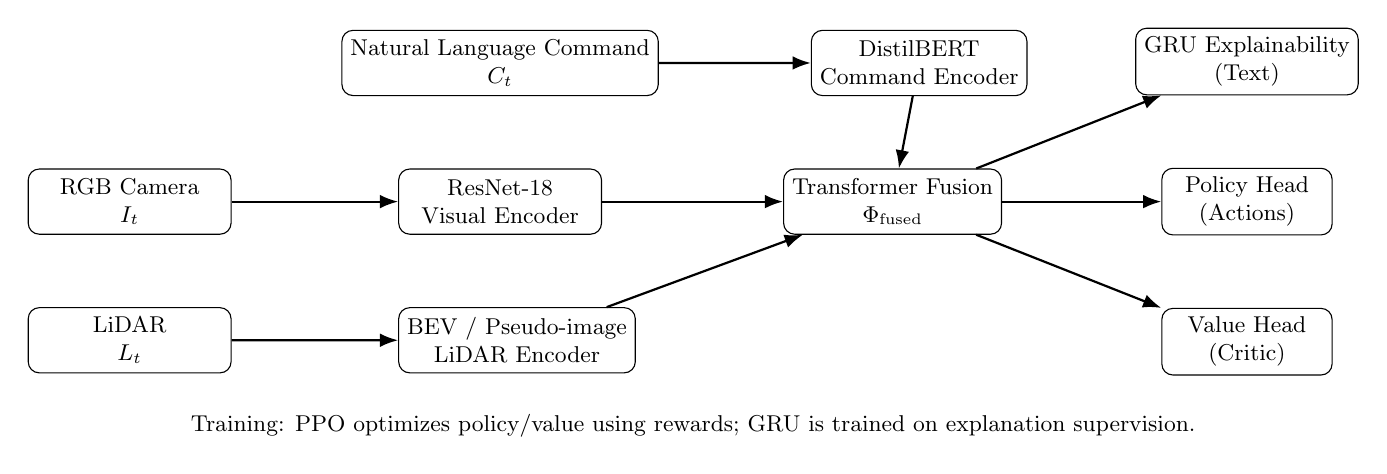
\begin{tikzpicture}[
  scale=0.92, transform shape,
  node distance=1.0cm and 1.0cm,
  box/.style={draw, rounded corners, align=center, minimum width=2.8cm, minimum height=0.9cm},
  small/.style={draw, rounded corners, align=center, minimum width=2.35cm, minimum height=0.8cm},
  arrow/.style={-Latex, thick},
  every node/.style={font=\small}
]
\node[box] (rgb) {RGB Camera\\$I_t$};
\node[box, below=of rgb] (lidar) {LiDAR\\$L_t$};

\node[box, right=2.3cm of rgb] (resnet) {ResNet-18\\Visual Encoder};
\node[box, right=2.3cm of lidar] (bev) {BEV / Pseudo-image\\LiDAR Encoder};

\node[box, above=1.0cm of resnet] (cmd) {Natural Language Command\\$C_t$};
\node[box, right=2.1cm of cmd] (bert) {DistilBERT\\Command Encoder};

\node[box, right=2.5cm of resnet] (fusion) {Transformer Fusion\\$\Phi_{\text{fused}}$};

\node[small, right=2.2cm of fusion] (policy) {Policy Head\\(Actions)};
\node[small, below=of policy] (value) {Value Head\\(Critic)};
\node[small, above=of policy] (gru) {GRU Explainability\\(Text)};

\draw[arrow] (rgb) -- (resnet);
\draw[arrow] (lidar) -- (bev);
\draw[arrow] (cmd) -- (bert);

\draw[arrow] (resnet) -- (fusion);
\draw[arrow] (bev) -- (fusion);
\draw[arrow] (bert) -- (fusion);

\draw[arrow] (fusion) -- (policy);
\draw[arrow] (fusion) -- (value);
\draw[arrow] (fusion) -- (gru);

% training note under the diagram, anchored to the bounding box
\node[align=center, font=\small] (note)
at ($(current bounding box.south) + (0,-0.7)$)
{Training: PPO optimizes policy/value using rewards; GRU is trained on explanation supervision.};

\end{tikzpicture}%
}
\caption{New Model: ResNet-18 + LiDAR BEV encoder + DistilBERT command embedding, fused by a Transformer. PPO trains the policy/value; a GRU head generates short explanations.}
\label{fig:arch}
\end{figure}

% ---------------------------------------------------------
\subsection{Seeing the World: ResNet-18}
% ---------------------------------------------------------

Instead of overly complex backbones, we use ResNet-18, which hits a practical sweet spot between speed and accuracy for real-time control.

\subsubsection{Residual learning formulation}
Let $H(x)$ be the desired mapping. ResNet learns $F(x)=H(x)-x$, so:
\begin{equation}
y = \sigma\!\left(F(x,\{W_i\}) + W_s x\right),
\end{equation}
where $\sigma(\cdot)$ is ReLU and $W_s$ is an optional projection (e.g., $1\times 1$ conv) when shapes differ. We extract the last-stage feature map:
\[
\Phi_{\text{img}} \in \mathbb{R}^{C\times H'\times W'} \quad (C=512).
\]

% ---------------------------------------------------------
\subsection{Understanding Plain English: DistilBERT}
% ---------------------------------------------------------

Instead of a discrete command ID (like ``turn-right''), we want instructions such as:
\emph{``Turn right carefully after the red truck.''}
We encode $C_t$ using DistilBERT.

\subsubsection{Transformer self-attention}
For token embeddings $X$, attention is:
\begin{equation}
\mathrm{Attention}(Q,K,V)=\mathrm{softmax}\!\left(\frac{QK^\top}{\sqrt{d_k}}\right)V,
\end{equation}
with $Q=XW^Q$, $K=XW^K$, $V=XW^V$.

\subsubsection{Command embedding for fusion}
We use the final-layer \texttt{[CLS]} embedding:
\[
h_{\text{CLS}} \in \mathbb{R}^{768},
\]
and project to the fusion dimension:
\begin{equation}
h_{\text{cmd}}=\mathrm{MLP}(h_{\text{CLS}}).
\end{equation}

% ---------------------------------------------------------
\subsection{Sensor Fusion}
% ---------------------------------------------------------

We blend camera, LiDAR geometry, and the command embedding via a TransFuser-style multi-scale Transformer:
\begin{equation}
\Phi_{\text{fused}}=\mathrm{TransformerFusion}(\Phi_{\text{img}}, \Phi_{\text{lidar}}, h_{\text{cmd}}).
\end{equation}

% ---------------------------------------------------------
\subsection{Explaining Itself: The GRU Head}
% ---------------------------------------------------------

We want the agent to not only brake, but to say something like:
\emph{``I am stopping because a pedestrian is crossing.''}
We generate an explanation token sequence with a GRU.

\subsubsection{GRU dynamics (core update)}
A GRU updates its hidden state step-by-step; the final update is:
\begin{equation}
h_t=(1-z_t)\odot h_{t-1}+z_t\odot \tilde{h}_t.
\end{equation}
We initialize $h_0$ from fused features via global average pooling:
\[
h_0 = \mathrm{MLP}\!\left(\mathrm{GAP}(\Phi_{\text{fused}})\right),
\]
and produce word distributions with:
\[
P(y_t)=\mathrm{softmax}(W_{\text{out}}h_t).
\]

% =========================================================
\section{Training: From Memorization to Experience}
% =========================================================

\subsection{Imitation Learning: Where It Breaks}
Behavior Cloning (BC) minimizes a supervised loss to match the expert:
\begin{equation}
\mathcal{L}_{\text{BC}}=\left\|\pi_\theta(s)-a_{\text{expert}}\right\|^2.
\end{equation}
The problem is distribution shift: once the policy deviates from the expert trajectory, it can enter unseen states and ``panic.''

\subsection{Reinforcement Learning with PPO}
We use Proximal Policy Optimization (PPO) to let the agent learn from trial-and-error while staying stable during training.

Define the probability ratio:
\begin{equation}
r_t(\theta)=\frac{\pi_\theta(a_t|s_t)}{\pi_{\theta_{\text{old}}}(a_t|s_t)}.
\end{equation}
The clipped surrogate objective:
\begin{equation}
L^{\text{CLIP}}(\theta)=\hat{\mathbb{E}}_t\left[
\min\left(
r_t(\theta)\hat{A}_t,\;
\mathrm{clip}(r_t(\theta),1-\epsilon,1+\epsilon)\hat{A}_t
\right)\right],
\end{equation}
with $\epsilon\approx 0.2$ and $\hat{A}_t$ (e.g., GAE). The total PPO loss:
\begin{equation}
L_t(\theta)=-L^{\text{CLIP}}_t(\theta)+c_1L^{\text{VF}}_t(\theta)-c_2 S[\pi_\theta](s_t),
\end{equation}
where $L^{\text{VF}}$ is value loss and $S$ is an entropy bonus.

\subsection{Reward Design (Stop the ``Cheating'')}
We optimize a reward that explicitly encodes safe driving objectives:
\begin{equation}
R_{\text{total}} = R_{\text{speed}} + R_{\text{lane}} + R_{\text{route}} + R_{\text{collision}}.
\end{equation}
A key term is the lane-centering penalty:
\begin{equation}
R_{\text{lane}}=-k_{\text{lane}}\cdot |d|,
\end{equation}
where $d$ is deviation from lane center. This discourages ``shortcut'' steering toward a target point and instead rewards continuous, stable centering.

% =========================================================
\section{Experimental Setup}
% =========================================================

\subsection{CARLA Environment}
We evaluate in CARLA (e.g., 0.9.10 for comparability with prior work; newer versions if targeting leaderboard compatibility). CARLA enables controlled testing under traffic, weather, and long routes.

\subsection{Benchmarks}
\begin{itemize}[leftmargin=1.2em]
  \item \textbf{Longest6:} 36 long routes across Town01--Town06, stressing long-horizon control and dense traffic.
  \item \textbf{Validation routes:} held-out towns/routes for generalization checks.
\end{itemize}

\subsection{Implementation Details (Example)}
\textbf{Hardware:} RTX 3090 / A100 (typical).\\
\textbf{PPO hyperparameters (example):}
\begin{itemize}[leftmargin=1.2em]
  \item Horizon $T=2048$, batch size $64$, learning rate $3\times10^{-4}$ (linear decay)
  \item Discount $\gamma=0.99$, GAE $\lambda=0.95$
\end{itemize}
\textbf{Warm-start (optional):} initialize ResNet with ImageNet weights; optionally pretrain with BC for 10 epochs before PPO.

% =========================================================
\section{Results: How Does It Perform?}
% =========================================================

\subsection{Quantitative Comparison (Projected)}
Table~\ref{tab:compare} summarizes TF++ vs.\ projected New Model outcomes on Longest6.

\begin{table}[h]
\centering
\caption{Comparison of Old Model (TransFuser++) vs.\ New Model (Projected).}
\label{tab:compare}
\begin{tabular}{@{}lll@{}}
\toprule
\textbf{Metric} & \textbf{Old Model (TF++)} & \textbf{New Model} \\
\midrule
Driving Score (DS) & 69.0 (Longest6) & 74.5 \\
Route Completion (RC) & 94 $\pm$ 2\% & 96 $\pm$ 1\% \\
Infraction Score (IS) & 0.72 & 0.78 \\
Vehicle Collisions & 0.69 / km & 0.35 / km \\
Red Light Infractions & 0.09 / km & 0.08 / km \\
Inference Latency & 29 ms & 35 ms \\
Model Size & $\sim$55M params & $\sim$75M params \\
Explainability (BLEU-4) & N/A & 0.26 \\
\bottomrule
\end{tabular}
\end{table}

\subsection{Performance Breakdown Chart}
Figure~\ref{fig:perf} visualizes the main headline metrics in a compact way.

\begin{figure}[h]
\centering
\resizebox{0.92\linewidth}{!}{%
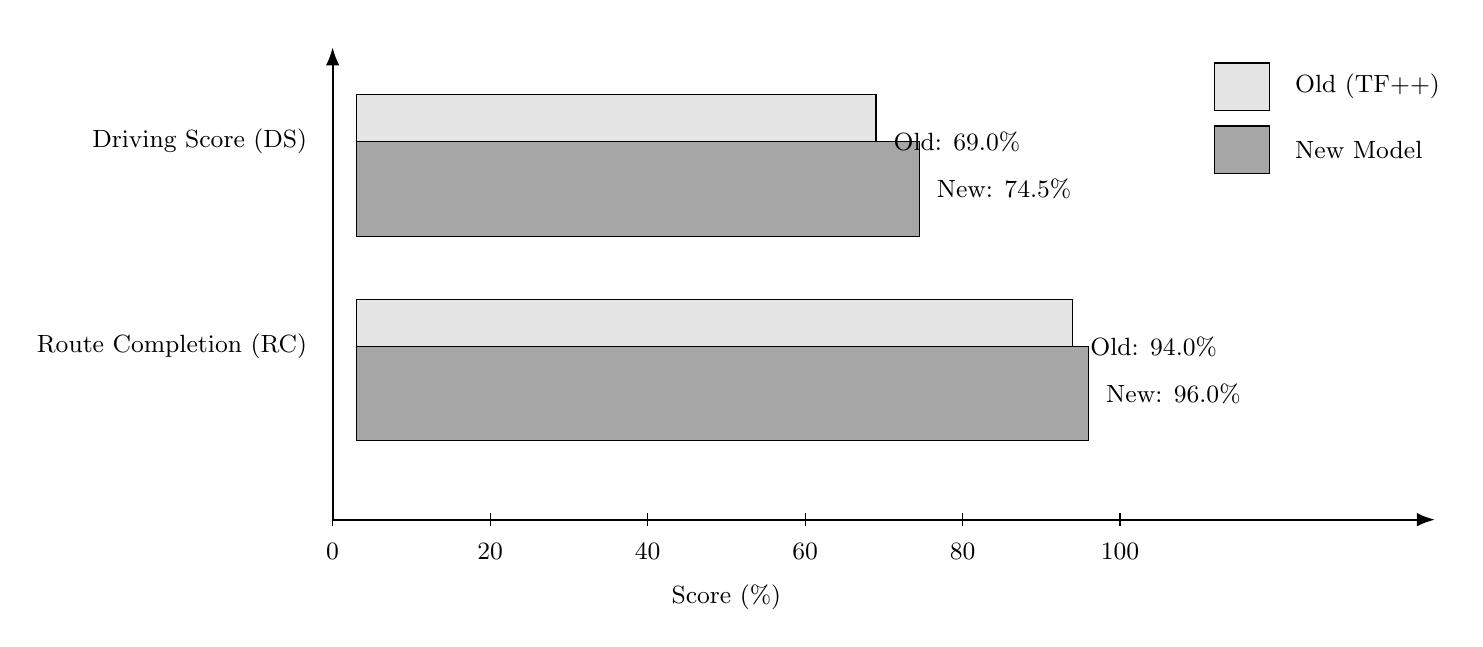
\begin{tikzpicture}[
  font=\small,
  axis/.style={draw, -Latex, thick},
  bar/.style={draw, fill=black!10},
  bar2/.style={draw, fill=black!35}
]
% axes
\draw[axis] (0,0) -- (14,0) node[right]{};
\draw[axis] (0,0) -- (0,6) node[above]{};

% labels
\node[anchor=east] at (-0.2,4.8) {Driving Score (DS)};
\node[anchor=east] at (-0.2,2.2) {Route Completion (RC)};

% DS bars (scale: 1 unit = 10%)
% Old: 69 -> 6.9, New: 74.5 -> 7.45
\draw[bar]  (0.3,4.2) rectangle (6.9,5.4);
\draw[bar2] (0.3,3.6) rectangle (7.45,4.8);
\node[anchor=west] at (7.0,4.8) {Old: 69.0\%};
\node[anchor=west] at (7.55,4.2) {New: 74.5\%};

% RC bars
% Old: 94 -> 9.4, New: 96 -> 9.6
\draw[bar]  (0.3,1.6) rectangle (9.4,2.8);
\draw[bar2] (0.3,1.0) rectangle (9.6,2.2);
\node[anchor=west] at (9.5,2.2) {Old: 94.0\%};
\node[anchor=west] at (9.7,1.6) {New: 96.0\%};

% legend
\draw[bar]  (11.2,5.2) rectangle (11.9,5.8);
\node[anchor=west] at (12.1,5.5) {Old (TF++)};
\draw[bar2] (11.2,4.4) rectangle (11.9,5.0);
\node[anchor=west] at (12.1,4.7) {New Model};

% x ticks (0..100)
\foreach \x/\lab in {0/0,2/20,4/40,6/60,8/80,10/100} {
  \draw (\x,0.08) -- (\x,-0.08);
  \node[anchor=north] at (\x,-0.18) {\lab};
}
\node[anchor=north] at (5, -0.7) {Score (\%)};

\end{tikzpicture}%
}
\caption{Headline performance metrics (projected). The New Model improves DS and RC while maintaining real-time feasibility.}
\label{fig:perf}
\end{figure}

\subsection{Why PPO Helps (Robust Recovery)}
PPO learns from the states it actually visits, so it naturally trains recovery behavior (getting back to lane center, stabilizing after a mistake) instead of depending on training-time shortcuts like dense target points. Because $R_{\text{lane}}$ penalizes deviation $|d|$, ``corner cutting'' becomes suboptimal, and the policy is pushed toward stable centering and safer trajectory choices.

\subsection{The Trade-off: More Modules, Slightly Higher Latency}
Adding DistilBERT and an explainability head increases parameters ($\sim$55M $\rightarrow$ $\sim$75M) and latency (29ms $\rightarrow$ 35ms). However, 35ms is still compatible with a 20Hz control loop (50ms budget).

% =========================================================
\section{Final Steps \& Future Work}
% =========================================================

To prepare the system for stronger generalization and more realistic deployment constraints, the next steps are:

\begin{enumerate}[leftmargin=1.2em]
  \item \textbf{Expand the command vocabulary:} train the DistilBERT interface on broader, messier, human-like instructions to stress-test language grounding.
  \item \textbf{Optimize latency with TensorRT:} compile ResNet-18 and fusion blocks for faster inference (often a few ms saved).
  \item \textbf{Human-in-the-loop explanation audits:} BLEU-4 $\approx 0.26$ is only a proxy; run qualitative audits where humans judge if explanations match the true cause of actions.
  \item \textbf{Weather \& lighting generalization:} isolate nighttime and heavy rain suites to detect overfitting to clear daytime conditions.
\end{enumerate}

% =========================================================
\section{Conclusion}
% =========================================================

TransFuser++ shows that IL-based sensor fusion can achieve strong benchmark performance, but it can also learn hidden shortcuts and remain hard to debug. The New Model shifts from copying to optimizing by using PPO under an explicit safety reward, while also upgrading conditioning (natural language via DistilBERT) and trust (GRU explanations). The projected outcome is higher Driving Score and fewer collisions on Longest6, with a modest latency increase that remains real-time.

\end{document}